\documentclass[
  bibliography=totoc,     % Literatur im Inhaltsverzeichnis
  captions=tableheading,  % Tabellenüberschriften
  titlepage=firstiscover, % Titelseite ist Deckblatt
]{scrartcl}

% Paket float verbessern
\usepackage{scrhack}

% Warnung, falls nochmal kompiliert werden muss
\usepackage[aux]{rerunfilecheck}

% unverzichtbare Mathe-Befehle
\usepackage{amsmath}
% viele Mathe-Symbole
\usepackage{amssymb}
% Erweiterungen für amsmath
\usepackage{mathtools}

% Fonteinstellungen
\usepackage{fontspec}
% Latin Modern Fonts werden automatisch geladen
% Alternativ zum Beispiel:
%\setromanfont{Libertinus Serif}
%\setsansfont{Libertinus Sans}
%\setmonofont{Libertinus Mono}

% Wenn man andere Schriftarten gesetzt hat,
% sollte man das Seiten-Layout neu berechnen lassen
\recalctypearea{}

% deutsche Spracheinstellungen
\usepackage{polyglossia}
\setmainlanguage{german}


\usepackage[
  math-style=ISO,    % ┐
  bold-style=ISO,    % │
  sans-style=italic, % │ ISO-Standard folgen
  nabla=upright,     % │
  partial=upright,   % ┘
  warnings-off={           % ┐
    mathtools-colon,       % │ unnötige Warnungen ausschalten
    mathtools-overbracket, % │
  },                       % ┘
]{unicode-math}

% traditionelle Fonts für Mathematik
\setmathfont{Latin Modern Math}
% Alternativ zum Beispiel:
%\setmathfont{Libertinus Math}

\setmathfont{XITS Math}[range={scr, bfscr}]
\setmathfont{XITS Math}[range={cal, bfcal}, StylisticSet=1]

% Zahlen und Einheiten
\usepackage[
  locale=DE,                   % deutsche Einstellungen
  separate-uncertainty=true,   % immer Fehler mit \pm
  per-mode=symbol-or-fraction, % / in inline math, fraction in display math
]{siunitx}

% chemische Formeln
\usepackage[
  version=4,
  math-greek=default, % ┐ mit unicode-math zusammenarbeiten
  text-greek=default, % ┘
]{mhchem}

% richtige Anführungszeichen
\usepackage[autostyle]{csquotes}

% schöne Brüche im Text
\usepackage{xfrac}

% Standardplatzierung für Floats einstellen
\usepackage{float}
\floatplacement{figure}{htbp}
\floatplacement{table}{htbp}

% Floats innerhalb einer Section halten
\usepackage[
  section, % Floats innerhalb der Section halten
  below,   % unterhalb der Section aber auf der selben Seite ist ok
]{placeins}

% Seite drehen für breite Tabellen: landscape Umgebung
\usepackage{pdflscape}

% Captions schöner machen.
\usepackage[
  labelfont=bf,        % Tabelle x: Abbildung y: ist jetzt fett
  font=small,          % Schrift etwas kleiner als Dokument
  width=0.9\textwidth, % maximale Breite einer Caption schmaler
]{caption}
% subfigure, subtable, subref
\usepackage{subcaption}

% Grafiken können eingebunden werden
\usepackage{graphicx}
% größere Variation von Dateinamen möglich
\usepackage{grffile}

% schöne Tabellen
\usepackage{booktabs}

% Verbesserungen am Schriftbild
\usepackage{microtype}

% Literaturverzeichnis
\usepackage[
  backend=biber,
]{biblatex}
% Quellendatenbank
\addbibresource{lit.bib}
\addbibresource{programme.bib}

% Hyperlinks im Dokument
\usepackage[
  unicode,        % Unicode in PDF-Attributen erlauben
  pdfusetitle,    % Titel, Autoren und Datum als PDF-Attribute
  pdfcreator={},  % ┐ PDF-Attribute säubern
  pdfproducer={}, % ┘
]{hyperref}
% erweiterte Bookmarks im PDF
\usepackage{bookmark}

% Trennung von Wörtern mit Strichen
\usepackage[shortcuts]{extdash}

\author{%
  AUTOR A\\%
  \href{mailto:authorA@udo.edu}{authorA@udo.edu}%
  \texorpdfstring{\and}{,}%
  AUTOR B\\%
  \href{mailto:authorB@udo.edu}{authorB@udo.edu}%
}
\publishers{TU Dortmund – Fakultät Physik}


\subject{v204}
\title{Wärmeleitung von Metallen}
\date{%
%  Durchführung: 7.11.2017
%  \hspace{3em}
%  Korrektur: 22.7.2017
\begin{align}
& \text{Durchführung: 7.11.2017} & \hspace{3em} & \text{Abgabe: } & {14.11.2017}\notag \\
& & &\text{Korrektur: } & \text{26.11.2017} \notag
\end{align}
}

\begin{document}

\maketitle
\thispagestyle{empty}
\tableofcontents
\newpage

\section{Zielsetzung}
Die Wärmeleitfähigkeit von Aluminium, Edelstahl und Messing soll untersucht werden.
\section{Theorie}
\label{sec:Theorie}
In einem Körper, welcher sich in einem Temperaturungleichgewicht befindet, kommt es zum Wärmetransport entlang des Temperaturgefälles.
Für Festkörper findet der Wärmetransport über Phononen und freie Elektronen statt.
Es wird ein Stab der Länge L und Querschnittsfläche A betrachtet.
Er besitzt die Materialdichte $\rho$ und spezifische Wärme $c$.
Die Wärmemenge,
\begin{equation}
  \label{eqn:gl1}
    \symup{d}Q =-  \kappa A \frac{\partial T}{\partial x} \symup{d}t,
\end{equation}
fließt in der Zeit $\symup{dt}$ durch die Querschnittsfläche $A$.
Das negative Vorzeichen deutet an, dass der Wärmestrom gemäß des zweiten Haupsatzes der
Thermodynamik in Richtung abnehmender Temperatur fließt.
Für die Wärmestromdichte gilt
\begin{equation}
    j_\omega =- \kappa \frac{\partial T}{\partial x}.
\end{equation}
Aus der Kontinuitätsgleichung ergibt sich die eindimensionale Wärmeleistungsgleichung
\begin{equation}
    \frac{\partial T}{\partial t} = \frac {\kappa}{\rho} \frac{\partial^2  T}{\partial x^2}.
\end{equation}
Sie beschreibt räumliche und zeitliche Entwicklung der Temperaturverteilung.
Die Temperaturleitfähigkeit
\begin{equation}
    \sigma_T = \frac{\kappa}{\rho c}
\end{equation}
gibt die Geschwindigkeit an mit welcher sich eine Temperaturdifferenz ausgleicht.
%
Eine Temperaturwelle der Form
\begin{equation}
    T\left(x,t\right) = T_\text{max}e^{\sqrt{\frac{\omega\rho c}{2 \kappa}}x} \cos\left(\omega t - \sqrt{\frac{\omega\rho c}{2 \kappa}}x\right)
\label{eqn:thermowelle}
\end{equation}
entsteht in einem sehr langen Stab durch periodischen Temperaturwechsel.
Ihre Phasengeschwindigkeit lautet:
\begin{equation}
    \upsilon = \sqrt{\frac{2\kappa\omega}{\rho c}}
\end{equation}
Für die Wärmeleitfähigkeit ergibt sich, mit  $\omega=\frac{2\pi}{T^*}$ und $\phi=\frac{2\pi\symup{\Delta}t}{T^*}$,
\begin{equation}
    \kappa = \frac{\rho c\left(\symup{\Delta}x\right)^2}{2 ln\left(A_\text{nah}/A_\text{fern}\right)\symup{\Delta}t}.
    \label{eqn:wleitfaehigkeit}
\end{equation}
Dabei ergibt sich die Dämpfung aus dem Amplitudenverhältnis $A_\text{nah}$ und $A_\text{fern}$ der Welle an zwei Messpunkten
$x_\text{nah}$ und $x_\text{fern}$.
$\symup{\Delta}t$ ist die Phasendifferenz der Welle zwischen den beiden Messpunkten und $\symup{\Delta}x$ ist der Abstand zwischen
diesen.

\section{Durchführung}
\label{sec:Durchführung}
Die verscheidenen Wärmeleitfähigkeiten werden mithilfe des folgenden Versuchsaufbaus \ref{fig:aufbau}
untersucht. Die Thermoelemente haben jeweils den Abstand \SI{30}{\milli\meter}.
\begin{figure}
    \centering
    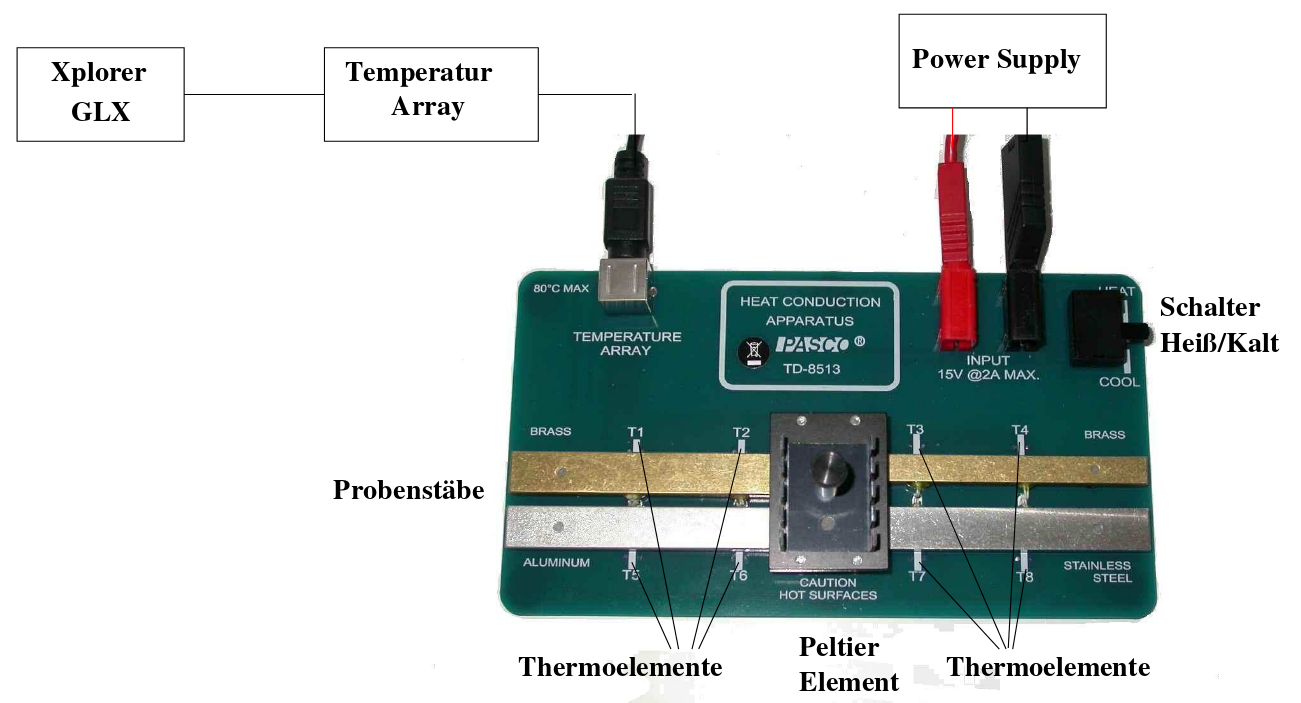
\includegraphics[width=\textwidth]{content/aufbau.png}
    \caption{Versuchsaufbau\cite{v204}}
    \label{fig:aufbau}
\end{figure}
Dabei heizt das Peltierelement die vier Metallstäbe simultan und die Temperatur wird an 8
verschiedenen Messpunkten, je zwei pro Stab, mithilfe vom Thermoelementen gemessen. Die
Messwerte werden über ein Temperature Array mit einem Datenlogger aufgezeichnet.
Die Maße der zu untersuchenden Metallstäbe sind:
\begin{table}
    \centering
    \caption{Abmessungen der Metallstäbe \cite{v204}}
    \label{tab:werte}
    \sisetup{table-format=3.0}
    \begin{tabular}{c c S[table-format=4.0] S S}
       \toprule
        {Material} & {Abmessungen$/\si{\centi\meter\cubed}$} &{$\rho/\si{\kg\per\meter\cubed}$} &{$c/\si{\joule\per\kg\per\kelvin}$} &{$\kappa/\si{\watt\per\meter\kelvin}$\cite{waermeleit}} \\
        \midrule
        Messing (breit) & $9 \cdot 1.2 \cdot 0.4$ & 8520 & 385 & 120 \\
        Messing (schmal) & $9 \cdot 0.7 \cdot 0.4$ & 8520 & 385 & 120 \\
        Aluminium (breit) & $9 \cdot 1.2 \cdot 0.4$ & 2800 & 830 & 237 \\
        Edelstahl (breit) & $9 \cdot 1.2 \cdot 0.4$ & 8000 & 400 & 15 \\
        \bottomrule
    \end{tabular}
\end{table}
%
\subsection{Statische Methode}
\label{sec:statische Methode}
Das Peltierelement wird mit $U_\text{P}=\SI{5}{\volt}$ betrieben.
Die vier Metallstäbe werden eine halbe Stunde lang erhitzt.
An den acht Thermoelementen wird die Temperatur gemessen und der jeweilige Wert alle 5 Sekunden gespeichert.
Anschließend werden die Stäbe durch das Peltierelement gekühlt.
%
\subsection{Dynamische Methode}
\label{sec:dynamische Methode}
Bei der dynamischen Methode, auch Angström-Verfahren, wird im Gegensatz zur statischen Methode nicht kontinuierlich,
sondern periodisch mit $U_\text{P}=\SI{8}{\volt}$ geheizt und gekühlt.
Der Datenlogger wird außerdem auf eine Abtastperiode von $\SI{2}{\second}$ gestellt.
Es ergibt sich innerhalb des Materials eine Temperaturwelle wie durch Gleichung \eqref{eqn:thermowelle} beschrieben.
In der ersten Messung werden zehn Perioden mit einer Periodendauer von $\SI{80}{\second}$ aufgezeichnet,
in der zweiten Messung ist etwa eine Stunde lang mit einer Periodendauer von $\SI{400}{\second}$ gemessen.

\section{Auswertung}
\label{sec:Auswertung}
\subsection{Statische Methode}
\begin{figure}
    \centering
    \includegraphics{plot.pdf}
    \caption{Temperaturverläufe der äußeren Thermoelemente}
    \label{fig:plot}
\end{figure}
Die Temperaturverläufe der äußeren Thermoelemente wurden in \ref{fig:plot} aufgetragen.
Auffallend ist, dass alle Graphen nach ungefähr 200 Abstraten ein Plateau aufweisen.
Die Temperatur der beiden Messingstäbe steigt jedoch langsamer an als die des Aluminiumstabes und schneller als die Temperatur des Edelstahlstabes.
%
Nach 700 Sekunden lässt sich dies schon beobachten.
Dort besitzen sie die follgenden Temperaturen:
\begin{table}
    \centering
    \caption{Temperaturen nach 700 Sekunden}
    \label{tab:t_1}
    \begin{tabular}{c c}
        \toprule
        $T$ & "Temperatur[Celsius]" \\
        \midrule
        1 & 27.5 \\
        4 & 26.5 \\
        5 & 28.5 \\
        8 & 24 \\
        \bottomrule
    \end{tabular}
\end{table}
\begin{figure}
    \centering
    \includegraphics{plot2.pdf}
    \caption{Temperaturdifferenz der Thermoelemente an Messing und Edelstahl}
    \label{fig:plot2}
\end{figure}
%
In \ref{fig:plot2} ist die Temperaturdifferenz nach der Zeit aufgetragen.
Die jeweiligen Graphen beziehen sich auf Messing- und Edelstahlstab.
Die Differenz steigt bei beiden erst rapide an.
Bei dem Messingstab fällt die kurve jedoch wieder stark ab und verläuft im späteren Verlauf nahezu waagerecht.
Die Temperaturdifferenz der Thermoelemente des Edelstahlstabes fällt nur langsam nach dem Maximum ab.

\section{Diskussion}
\label{sec:Diskussion}
Anhand der Information die aus der statischen Messmethode gewonnen werden, lässt sich eine erste Abschätzung über die Wärmeleitfähigkeit der verschiedenen Materialien machen.
Nach 700 Sekunden ist bereits ersichtlich, dass sich der Aluminiumstab am schnellsten erwärmt.
Folglich sollter dieser die größte Wärmeleitfähigkeit besitzen.
Am zweitschnellsten erwärmt sich Messing unabhängig von seinem Durchmesser.
Dabei ist jedoch zu beachten, dass der Wärmestrom stärker ist bei größerem Durchmesser.
Die Temperaturdifferenz bei Edelstahl ist größer als diese bei Messing, was auch durch die Wärmeleitfähigkeit bedingt ist.
Aus \ref{tab:3} wird erkenntlich, dass der Wärmestrom unabhangig von der Temperatur des Materials ist.

Mithilfe der dynamischen Methode kann die Wärmeleitfähigkeit nicht nur qualitativ, sondern auch quantitativ bestimmt werden.
Jedoch ist die dazu notwendige Bestimmung der Amplituden und Phasenverschiebungen durch Ablesen am Graphen sehr mühsam und fehlerbehaftet.
Die starken Abweichungen zu den Literaturwerten können einerseits durch die fehlerbehaftete 
Messmethode, andererseits aber auch dadurch erklärt werden, dass die genaue Legierung der 
Metalle nicht bekannt ist.
Durch die Angström-Methode lassen sich die Erkenntnisse der statischen Methode bestätigen und genauer konkretisieren.


\nocite{*}
\printbibliography{}

\end{document}
